\documentclass[10pt,a4paper]{article}
\usepackage{vmargin}
\setpapersize{A4}
\setmargins{2.5cm}  % margen izquierdo
{1.5cm}             % margen superior
{16.5cm}            % anchura del texto
{23.42cm}           % altura del texto
{10pt}              % altura de los encabezados
{1cm}               % espacio entre el texto y los encabezados
{0pt}               % altura del pie de página
{2cm}               % espacio entre el texto y el pie de página

\usepackage[utf8]{inputenc}
\usepackage{amsmath}
\usepackage{amsfonts}
\usepackage{amssymb}
\usepackage{graphicx}
\usepackage{colortbl}
\usepackage{xcolor}
\usepackage{multirow, array} % per a les taules
\usepackage{fancyhdr}
\usepackage{tikz}
\usepackage{wrapfig}
\usepackage[toc,page]{appendix}
\usepackage{float}
\usepackage{todonotes}

\makeatletter
\newenvironment{varappendices}[2]% #1 is the global name, #2 the single name
 {\renewcommand{\appendixpagename}{#1}%
  \renewcommand{\appendixtocname}{#1}%
  \renewcommand{\appendixname}{#2}%
  \addtocontents{toc}{\protect\setcounter{tocdepth}{2}}%
  \addtocontents{toc}{%
    \begingroup
    \let\protect\l@chapter\protect\l@section
    \let\protect\l@section\protect\l@subsection
  }%
  \appendices
  \setcounter{chapter}{0}}
 {\addtocontents{toc}{\endgroup}%
  \endappendices}

\title{<++>}
\author{<++>}
\date{September 2020}

\definecolor{Gris}{gray}{0.9} % Color tablas
\definecolor{gris}{HTML}{DDDCD0} % Color tabla de nombres
\definecolor{rosat}{HTML}{FCD2C1} % Color título inicial
\definecolor{separador}{HTML}{C9A704} % Color de les líneas separadores i del título de sección

\renewcommand{\appendixname}{Anexos}
\renewcommand{\appendixtocname}{Anexos}
\renewcommand{\appendixpagename}{Anexos}

\begin{document}

\parbox{3cm}{
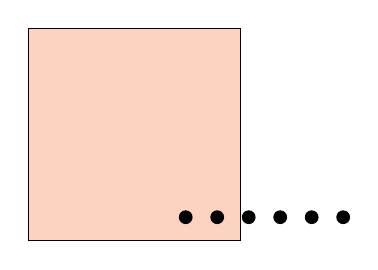
\begin{tikzpicture}
	% Quadrat
	\draw [fill=rosat](0,0) rectangle (2.7,2.7);
	% círculo:
	\draw [fill=black](2,0.3) circle (0.08cm);
	\draw [fill=black](2.4,0.3) circle (0.08cm);
	\draw [fill=black](2.8,0.3) circle (0.08cm);
	\draw [fill=black](3.2,0.3) circle (0.08cm);
	\draw [fill=black](3.6,0.3) circle (0.08cm);
	\draw [fill=black](4,0.3) circle (0.08cm);
\end{tikzpicture}
}
\parbox{6cm}{\huge Práctica <++>: \\ <++>}
\vspace{5mm} %5mm vertical space

\begin{tabular}{|>{\columncolor{gris}} l|l|}
	\hline
	Nombre y Apellidos & <++> \\ \cline{1-2}
	Nombre y Apellidos & <++> \\ \cline{1-2}
\end{tabular}
\vspace{5mm} %5mm vertical space

\begin{tabular}{| l|l|}
	\hline
	Número de grupo de laboratorio & <++> \\ \cline{1-2}
\end{tabular}

\vspace{4mm} %5mm vertical space
{\color{separador} \rule{0.5\linewidth}{0.7mm} }

\section*{\color{separador} Preguntas}
<++>

\begin{enumerate}
    \item <++>

\end{enumerate}


\newpage
\appendix
%\appendixpage
%\addappheadtotoc
\begin{appendices}
\section*{Anexo <++>}\label{anexo <++>}
\subsection*{<++>}

\newpage
\section*{Anexo <++>}\label{anexo <++>}
\subsection*{Caso B}

\end{appendices}

\end{document}
